\chapter{Costantini - Pirotte}

	3 octobre : Celso COSTANTINI, Réforme des missions au XXe siècle, Casterman, 1960, p. 237-246 et Jean PIROTTE, « Mise en perspective. Images et vie chrétienne. Quels liens ? Pour quel message », dans J. PIROTTE, Caroline SAPPIA et Olivier SERVAIS (dir.), Images et diffusion du christianisme. Expressions graphiques en contexte missionnaire XVIe-XXe siècles, Paris, Karthala, 2012, p. 19-42. \sn{personnage atypique : pourquoi les nouvelles Eglises n'ont pas leurs propres Eveques ? Eglise dans la culture locale. Pirotte : article qui complète les écrits de C. Constantini sur la place des images}


\section{Celso COSTANTINI, Réforme des missions au XXe siècle}

\paragraph{1960} Chine
Après la première guerre mondiale, nouveau modèle avec des prêtres indigènes. 1919 : \textit{Maximud Illium}. puis \textit{Rerum Ecclesiae}. 

Séminaire en 1899, vice chancelier de la conférence épiscopale. 1919 : directeur du musée d'Apimée (?), intéret pour la culture. Eveque en 1921, en Chine en 1922, \textit{délégué apostolique}. 

\paragraph{1924 premier concile de Shanghai} En 1926, évêques Chinois.

\paragraph{1933 : retour à Rome pour raison de santé} 1953 cardinal. Mort en 1958

\begin{Synthesis}
    Application de la réforme des missions en Chine
\end{Synthesis}



\paragraph{Evangéliser et non coloniser} 

\begin{singlequote}
détruisez les idoles mais non les temples
St Augustin de Canterbery
\end{singlequote}

\paragraph{respecter la culture et l'art du pays évangélisé }

\begin{singlequote}
    Etoile polaire des missions. Pie XII.
\end{singlequote}


\paragraph{dépouiller l'art sacré des formes étrangères}
D'abord extremement sévère (cf Pekin : caractère étranger et irrespectueux par rapport à la cité interdite). 

\begin{singlequote}
    Il lui manque le courage l'originalité, l'esprit qui animaient les anciens et c'est pourquoi il ne crée plus de grandes oeuvres.
\end{singlequote}

Mais un mouvement positif : \textit{adaptation}. Dans tous les pays de mission, un printemps d'art autochtone.
Université catholique de Pekin






\paragraph{Question sur }

\begin{singlequote}
    241 -Le christianisme est une idée force: ce n'est pas lui qui doit s'adapter
à l'architecture chinoise ou indienne; c'est cette architecture qui
doit s'adapter au catholicisme. 
\end{singlequote}
 Cite bcp Th. Ohm, bénédictin. \href{https://de.wikipedia.org/wiki/Thomas_Ohm}{Thomas Ohm sur Wikipedia}
 
\paragraph{Néogothique / néo Romane} La critique néogothique est dure. Derrière ce \textit{néo}, il y a une volonté de revenir à l'unité chrétienne au XIXème (romantisme au XIII).

\paragraph{Figuratif oeuvre à spiritualité}

\paragraph{Minorité chrétienne face à la majorité non croyante} Les croyants peuvent être sensibles à l'art occidential mais la majorité ? que voit elle ?

\paragraph{Chant chinois proche du Grégorien ?}

\subsection{réflexions personnelles}

\paragraph{CR de travaux pratiques ? } On a affaire à quelqu'un qui a de la matière sur quoi il parle
\paragraph{bcp de portes ouvertes  : est ce la cas à l'époque}


\paragraph{Il y a un impensé : trouver le christianisme de façon pure hors de la culture chrétienne } Comment on implante un message, l'Evangile déjà inculturé dans la culture "occidentale". 


\section{Jean PIROTTE, « Mise en perspective. Images et vie chrétienne. Quels liens ? Pour quel message »}

\paragraph{mise en perspective : on va regarder différents domaines}

\paragraph{Jean Pirotte} Historien Belge. 
Transmission du Catholicisme par les images.




Pourtant, le simple usage pastoral de l'expression esthétique pour ame­ ner à croire n'explique pas totalement cette connivence entre les religions et les images


\paragraph{
Une arme dans l'arsenàl de l'éducation à la foi
}

\subparagraph{rejet de L'image, « docteur des ignorants » ? }

Ces images situées loin des yeux des fidèles, images par ailleurs complexes et exigeant un long décodage, se prêtaient-elles vraiment à la rumination individuelle des mystères religieux par les gens simples ou à une catéchèse habituelle ? On peut en douter. 
Permettant de fixer des pensées pieuses sur un objet de dimension réduite, l'image fut utilisée par les agents de la Contre-Réforme, notam­ ment les Jésuites, comme un outil de premier choix. 


\paragraph{Le décor du paysage mental catholique} contre reforme

\paragraph{Images d'une chrétienté qui s'exporte
}
De même, de nos jours, les convertis occidentaux au bouddhisme se sentent-ils davantage bouddhistes lorsqu'ils revêtent la longue robe safran ou amarante en agitant l'un ou l'autre ustensile du lamaïsme tibétain ? 

la figure forte d'une antithèse opposant
1 avant al après, le <sans» à l' «avec» (opposition entre la dégradation du monde s s la foi, sans le missionnaire et les merveilles opérées par la grâce sous l influence chrétienne)19


\paragraph{La menace du Kitsch : un péril pour l'Eglise catholique ?} Plus que toute autre forme d'expression artistique, l'image religieuse serait-elle menacée par le kitsch \sn{21.	Sur le kitsch, voir l'ouvrage d'Abraham A. MOLES, Le kitsch.- l'art du bonheur, Pa­ ris, 1971. Voir aussi: Kitsch. An anthology of bad taste, sous la dir. de Gillo DORFLES, Londres, 1969.}? Ne s'agirait-il pas d'un mal nécessaire? Une religion qui rejette les tendances puristes et sectaires pour s'ouvrir au plus grand nombre est amenée à mettre l'art qu'elle inspire à la portée des masses ; elle devra de ce fait tolérer des imperfections dans la diffusion des copies. La typologie de l'Église et de la secte établie par le sociologue allemand Ernst Troeltsch est éclairante à ce sujet : par opposition aux groupes sectaires soucieux de purisme et se développant en marge de la société, le type «Église» s'adresse à la multitude, ressent la nécessité du compromis et s'ouvre davantage à la culture ambiante en vue de l' intégrer \sn{22.	D'après Troeltsch, par opposition au type « secte», seul le type «Église» est à même d'agir fortement sur les masses. Voir E. TROELTSCH, « Die Soziallehren der christli­ chen Kirchen und Gruppen », Tübingen, 1912 ; les conclusions ont été traduites en fran­
çais : Christianisme et société, dans Archives de sociologie des religions, n°l l, 1961, p. 15- 34.}.


\paragraph{image comme outil de propagande au XIX}


\subsection{Les images et les religions : de l'amour au rejet}
il reste qu'une parenté profonde unit les religions et les images : une relation étroite, où s'expriment alternativement l'amour et la haine.

\paragraph{L'ambivalence des images} comme le langage.

Il est vrai que certaines religions ont proscrit les représentations ima­ gées, considérées comme des tentations séductrices conduisant à la vénéra­ tion idolâtrique d'« images taillées» de la divinité que l'on ne peut enfer­ mer dans une fabrication humaine. À moins que ce ne soit l'homme lui­ même qui, aimant se contempler 

Théologie musulmane. 
Il est curieux de remarquer que les premiers signes connus de cette interdiction de la figuration dans l'islam remontent au début du VIIIe siè­ cle, quelques années seulement avant l'explosion de l'iconoclasme chré­ tien dans l'empire byzantin.


\paragraph{En Orient : une théologie de la beauté} À coup sûr, il s'agit d'une réaction de la pureté mono­ théiste contre la matérialisation du sacré dans l'image

On perçoit dans le discours de Jean Damascène des influences néoplatoniciennes, notamment le souffle de la théorie centrale de l'émanation: toutes choses procèdent de l'Un et s'animent d'un mouvement de retour vers leur source.

\paragraph{En Occident : la chasse aux déviations}

En Occident, l'iconophobie fut moins virulente. On retrouve des mani­ festations iconoclastes au moyen âge, notamment en Angleterre avec John Wycliff (vers 1320-1384) et ses Lo/lards, dénonçant le danger d'idolâtrie mais aussi la dérive vers l'ornementation luxueuse des églises alors que les communautés devaient se tourner vers les pauvres30. La Réforme protes­
tante du xvr siècle manifeste aussi de la méfiance vis-à-vis des images,
dans la mesure où elles apparaissent liées au culte des saints et aux objets supports des dévotions. Niant toute acquisition de la sainteté par les œu­ vres, les réformateurs ne pouvaient éprouver que de la crainte devant un univers d'objets et d'images aux forts relents de manipulation du divin:

Dans le monde catholique, à la même époque, on insiste alors sur le fait que l'image n'a pas de valeur cultuelle propre. 


\paragraph{manger les images

}




\subsection{réflexions personnelles}

\paragraph{lien particulier à l'image du christianisme} Nicée 2. Mais même pour le christianisme, on pourrait souligner l'homme défiguré puis l'ascension. d'une certaine manière, où est elle ? Il y a toujours une tension. On ne peut plus saisir l'image.

\paragraph{Balthazar : l'esthétique est subverti par la croix} Il y a des croix terribles. 

\paragraph{Iconostase} image du paradis, portes royales. A droite, vêtement rouge et bleu du Christ. A gauche, mere de Dieu, vétement de bleu recouvert de rouge. 

\paragraph{Image, à la fois vecteur de communication et image mentale} sur l'image mentale, on ne change pas facilement d'image. COmment un africain pense palestine ? 


\section{compte rendu}
\sn{Jean-Christophe NORMAND}


Compte-rendu de séance du 3 octobre 2023
Textes travaillés :
1.	Réforme des missions au XXe siècle (Cardinal C. Costantini) – extraits
2.	Mise en perspective – images et vie chrétienne – quels liens, pour quel message ? de Jean Pirotte


Notre thème de la semaine dernière portait sur le rapport à l’image du point de vue de la mission et plus largement des religions. Pour cela nous avons lu deux textes : un extrait de Réforme des missions au 20e s du Cardinal Costantini et une mise en perspective du rapport entre images et vie chrétienne de l’historien belge Jean Pirotte publié dans le cadre d’un colloque du CREDIC dont la mission est en particulier d’associer des universitaires, des acteurs de la mission et des personnes qui réfléchissent à l'inculturation du christianisme.

\paragraph{indigénisation}
Le premier auteur s’exprimait en tant que prélat avec une solide expérience de la mission en Chine dans les années 1920. Nous avons relevé la richesse de son témoignage et, en particulier de sa contribution active à l’indigénisation (terme peu usité aujourd’hui mais qui traduit bien son propos) du clergé en Chine, initiative relayée et appuyée par le pape Pie XI (ordination de 6 premiers évêques chinois en 1926). Nous avons compris également comment la vocation missionnaire de l’Église et l’inculturation de la foi chrétienne posaient des questions de sensibilité artistique et de capacité des cultures à entrer en dialogue les unes avec les autres. En particulier, le modèle colonial occidental (situation légations dans le cas de la Chine) du fait d’une confusion des intérêts, a pu se montrer contre-productif pour l’évangélisation des peuples faute de lieux de cultes adaptés et par manque d’un clergé indigène.

Nous avons relevé de nos lectures respectives les quelques points suivants :

\begin{marginfigure}
    \caption{Les concessions internationales : les Eglises ont été associées à ces concessions. }
    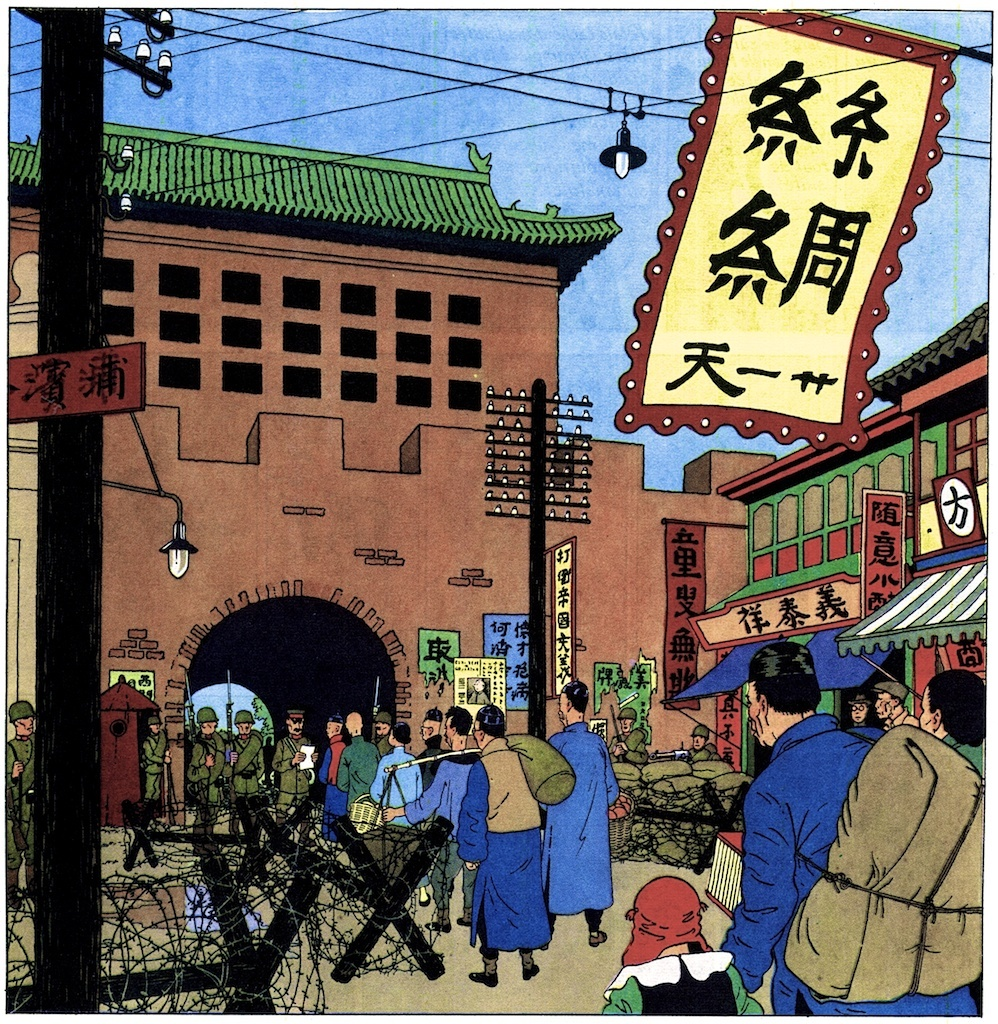
\includegraphics[width=\textwidth]{2023 - Dialogue Mission XX/Images/Sortie-de-l-enceinte Concession internationale.jpg}
\end{marginfigure}
\begin{itemize}
    \item Une forme de tension entre ces efforts d’inculturation à mener et en même temps la volonté d’honorer la tradition chrétienne occidentale dans sa manière de prier et de célébrer. Nous avons cité le texte conciliaire Sacrosanctum Concilium qui promeut la tradition des rites latins et du chant grégorien propre à l’occident, toute traduction devant être approuvée par l’autorité ecclésiastique du lieu (Cf SS §36).
        \item L’apport d’idées du père bénédictin allemand contemporain Thomas Ohm, cité à plusieurs reprises par l’auteur (Cf pages 239 et 241). Spécialiste en missiologie, il vient en appui (ou influence ?) dans l’orientation de la pensée critique de l’auteur sur les formes européanisantes des églises construites en Chine et la réplication d’un art occidental pauvre en comparaison de la culture millénaire chinoise.

            \item Un constat que les convictions de l’auteur ne dataient pas d’hier : déjà St Grégoire le Grand avait mis en garde contre une manière d’évangéliser qui ne prendrait pas en compte les coutumes locales. Ensuite, il a été rappelé que les principes mis en avant par le Cardinal avaient déjà été explicités au 17e siècle avec des instructions adressées par les Missions Étrangères de Paris sur l’importance du respect des cultures locales et la non-implication dans les décisions politiques engagées par les pouvoirs sur place (Cf les instructions par la Sacre Congregatio de Propaganda Fide du 10.11.1659 et notamment le §12 sur le respect des coutumes locales). Cela n’empêchera pas les conflits, selon l’auteur qui cite l’épisode de la querelle des rites au 18e. (p.239).

                \item Nous nous sommes étonnés de l’impensé que constituait la croyance que la religion chrétienne puisse être transposée telle quelle dans une autre culture : à la page 238 un extrait d’une audience publique de Pie XII en 1944 explique que « le missionnaire n’a pas mission de transplanter la civilisation européenne dans les pays de mission mais bien de disposer les peuples à accueillir et assimiler les éléments de vie et mœurs de vie chrétienne »). Nous avons relevé ici l’impossibilité de transplanter sans modifier la culture réceptrice et vice et versa. Il n’y a pas de message chrétien qui ne se rattache à une culture source. En général l’assimilation se fait toujours dans le sens de la culture dominante.

\end{itemize}
 


 

Le second texte de J.Pirotte nous a permis d’approfondir la question du rapport à l’image. Nous avons relevé comment l'image sert à exprimer l’« indicible» au sens étymologique (ce qui ne peut être dit par des mots) et vient ainsi au secours du langage religieux. L’image est ainsi décrite comme « un puissant outil d'enracinement de l'être humain dans le monde », « un système de médiation avec le sacré » (Cf page 20), ce qui explique le recours abondant à l’iconographie dans toutes les religions.
 



En même temps ce rapport à l’image est fortement ambivalent avec le risque d’idolâtrie souvent dénoncé – (Cf pages 28-36) en particulier chez le judaïsme et l’islam. Le christianisme fait figure d’exception, même s’il a été également secoué par des crises iconoclastes au 8e-9e siècles car il reprend à son compte la doctrine de l’incarnation (Dieu qui s’est fait homme). Dans la religion orthodoxe, l’image devient même théophanie (sacramentalisation de l’image). Mais de quelle image parlons-nous après la passion du Christ et de sa résurrection ? Comment restituer encore sa présence sous la forme des espèces eucharistiques ou de l’Esprit Saint. ? La dévotion aux images saintes ou aux représentations de la vie publique du Christ, sont-elles une juste exposition de la formulation de la foi chrétienne ?

Quelle que soient leurs utilisations, l’auteur nous montre comment les images sont d’abord au service des religions en s’installant dans une relation de connivence (l’image vient au secours du discours religieux). Dans cette mise en perspective, nous constatons une suite de rapports complexes et fluctuants de l’image aux religions selon les périodes. En post modernité, que nous dit l’image du religieux ? L’indicible pourrait-il être en réalité de l’ordre de l’incompris pour la majorité des contemporains ? Si sa vertu fondamentale est d’ouvrir au transcendantal, encore faut-il avoir les clés de lecture pour pouvoir les recevoir et les interpréter dans son contenu catéchétique et/ou théologique.
